\chapter{Klasifikacija}
\label{ch:klasifikacija}

V prešnjih lekcijah smo raziskali in gručili podatke, sedaj pa bi želeli zgraditi napovedni model. Tokrat bomo iz stopnje izraženosti genov poskusili napovedati funkcijo gena. Za to bomo uporabili podatke \textit{brown-selected.tab} iz Orangeve dokumentacije. Nato bomo gradnik \widget{File} povezali z gradnikom \widget{Predictions}.

Predictions sam po sebi ne pokaže ničesar. Potrebuje namreč še model - nekakšna navodila, kako naj napoveduje iz podatkov. Pripeljmo v Predictions še gradnik \widget{Tree}, kot vidite spodaj.

\begin{figure}[h]
    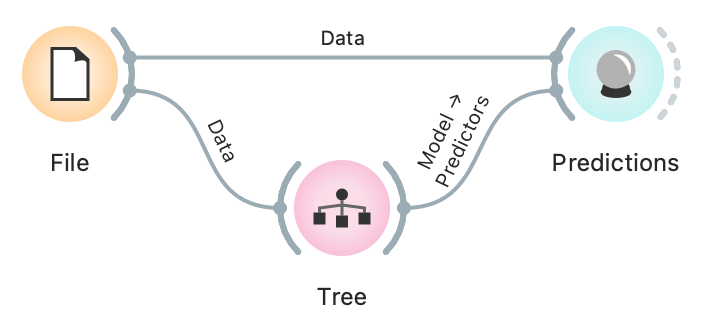
\includegraphics[width=0.8\linewidth]{workflow.png}%
    \caption{$\;$}
\end{figure}

Podatki pridejo v Tree, ki na podlagi podatkov zgradi napovedni model. Predictions dobi podatke iz gradnika File, iz gradnika Tree pa model. To je nekaj novega; v prejšnjih delotokih so si gradniki pošiljali zgolj podatke, tukaj pa imamo kanal, ki pošilja model.

Predictions uporabi model za izdelavo napovedi na podatkih in te napovedi prikaže v tabeli.

Kako točne so napovedi? Je ta model dober? Kako vemo?
Še prej pa - kaj sploh je drevo (Tree)? Kako izgleda? In kako ga Orange zgradi? Je to dober način gradnje algoritmov?

\begin{figure*}[h]
    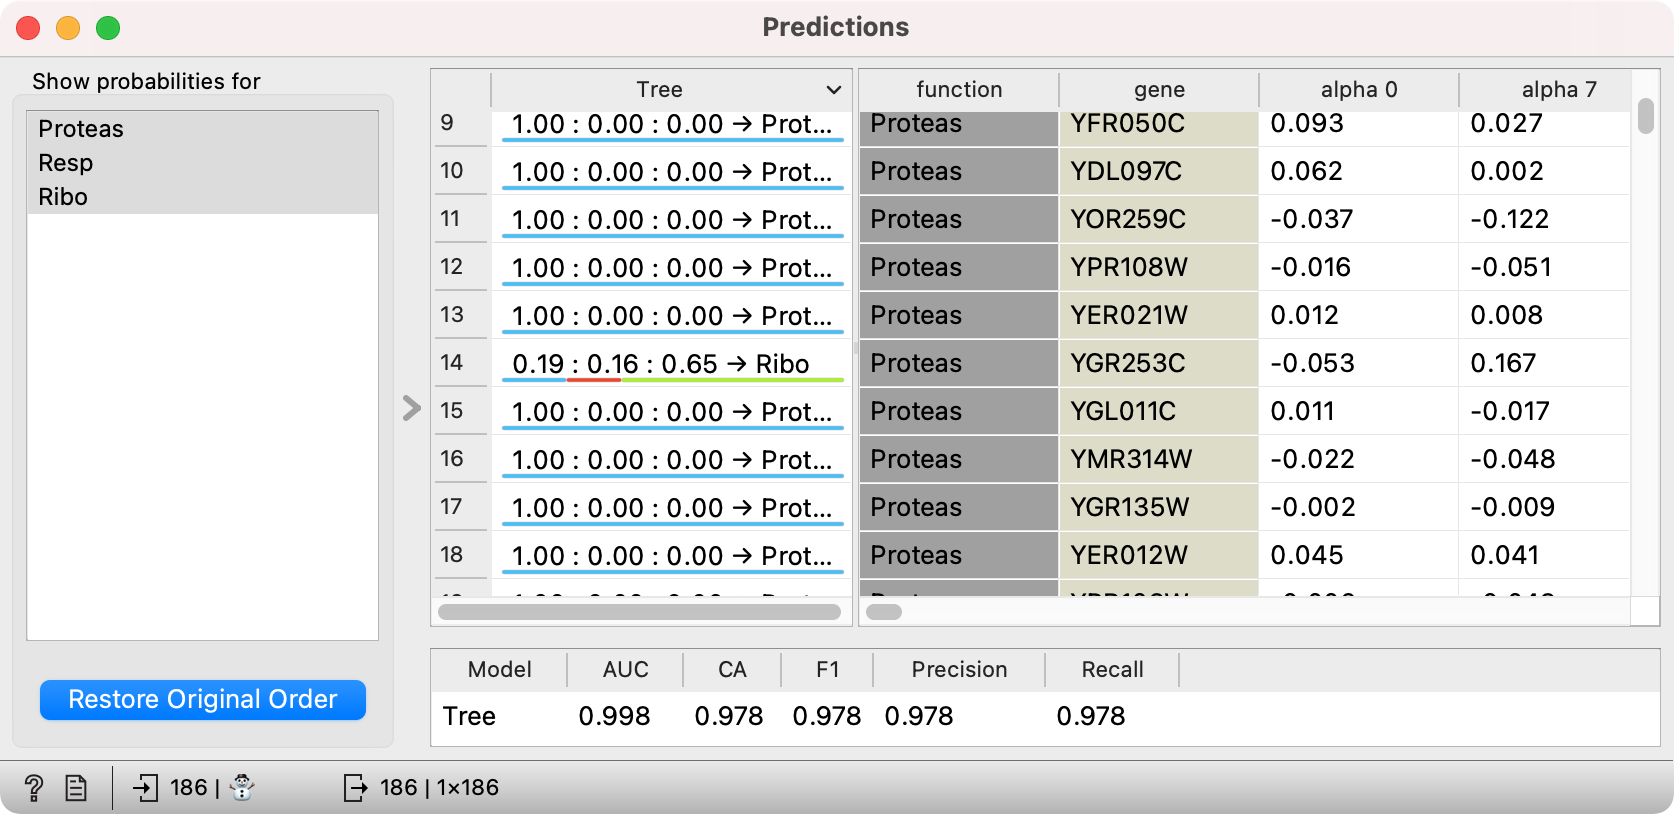
\includegraphics[width=0.8\linewidth]{predictions.png}%
    \caption{$\;$}
\end{figure*}
